\section{Method}
\label{sec:method}

\begin{figure}[t]
  \centering
  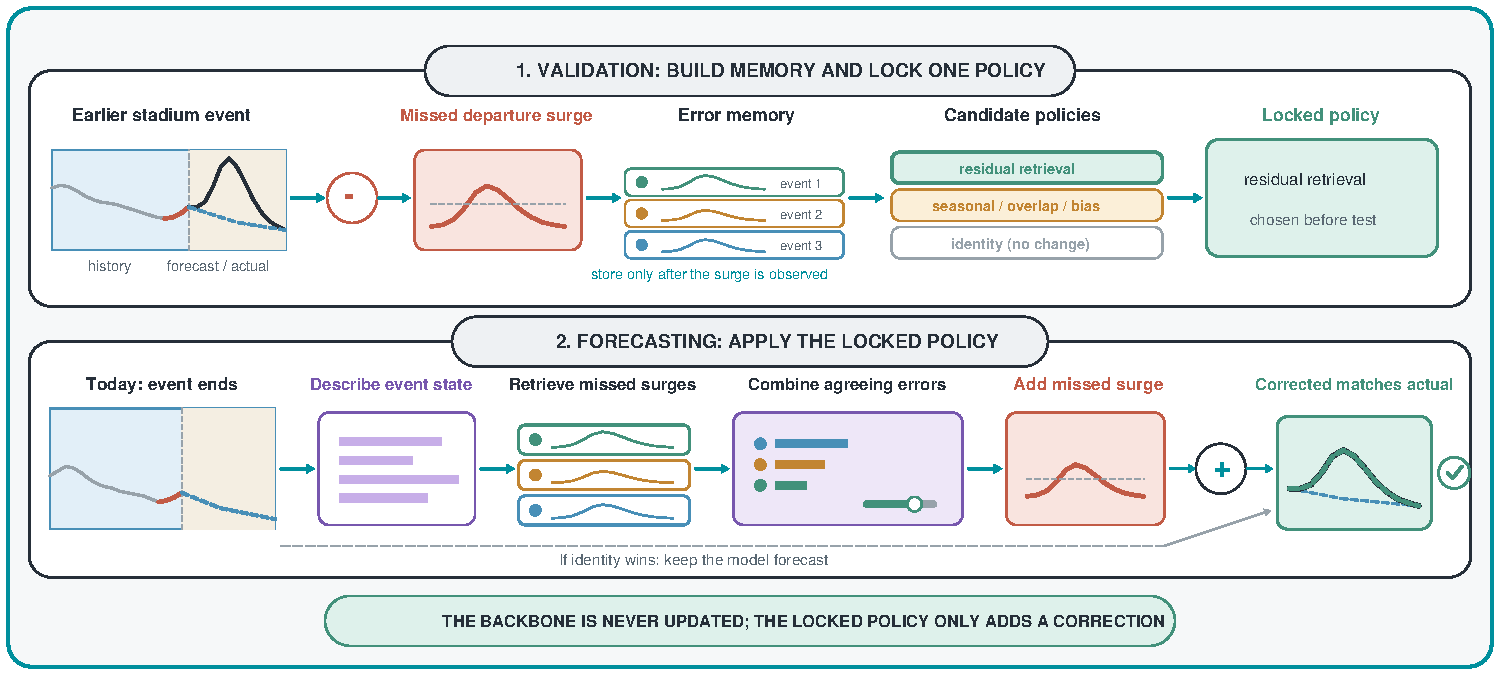
\includegraphics[width=0.82\textwidth]{figures/method_overview.pdf}
  \caption{\textbf{\method{} separates validation-time calibration from
  forecast-time correction.} On a held-out validation split, the forecaster's own
  predictions are differenced against realized targets to build an error memory, and one
  correction policy is locked. At forecast time the backbone is never updated: the
  locked policy either retrieves agreeing past errors and adds them to the
  current forecast, or falls back to a simpler correction, or leaves the
  forecast unchanged. The actual continuation is never available at forecast
  time.}
  \label{fig:method}
\end{figure}

\method{} has three components, sketched in Figure~\ref{fig:method}: a
chronological memory of a trained forecaster's own errors
(Section~\ref{sec:memory}), a model-conditioned retriever that turns them into a
reliability-shrunk correction whose \emph{object} is itself tunable
(Section~\ref{sec:retrieval}), and a validation gate that decides whether to apply
it (Section~\ref{sec:selection}).

\subsection{Retrieving errors instead of inputs}
\label{sec:memory}

\paragraph{Why the error is the right default object.}
The dominant design scores past windows by context similarity and reuses the
futures that followed
\citep{tire2024raf,han2025raft,lee2026crossrag,kang2026craft,zhou2026saraf}.
Storing $\resid_i$ instead of $\ytrue_i$ fixes three properties of that object.
Raw-window distance is dominated by the periodic and trend energy the base forecast
already predicts, so the short prefix announcing an unusual continuation rarely
decides the neighbourhood, whereas a residual has that explained component
subtracted out. A retrieved future is an absolute trajectory carrying its own level,
phase, and covariate response, so injecting it overwrites parts of $\ybase_t$ that
were already correct, while a residual can only move the forecast. And an input
neighbourhood is identical for every forecaster, whereas memory indexed to one
forecaster suppresses the correction when that backbone has no recurring error.
Appendix Figure~\ref{fig:residual-example} shows all three effects on measured ETTh1
forecasts: neighbours with matching contexts have futures at visibly different
levels, but their residuals share one error shape.

\paragraph{The two objects are one family.}
Retrieving a future and retrieving an error are not alternatives; they are the
two ends of a single additive correction. Anchoring neighbour $i$'s future to the
query endpoint, as input retrieval does, and subtracting the base forecast gives
an exact decomposition,
\begin{equation}
  \big(\ytrue_i + \shift_i\big) - \ybase_t
  \;=\;
  \resid_i + \drift_i,
  \qquad
  \drift_i = \ybase_i + \shift_i - \ybase_t,
  \qquad
  \shift_i = \xctx_{t,L} - \xctx_{i,L},
  \label{eq:objects}
\end{equation}
where $\xctx_{t,L}$ is the final context step. The left side is what input
retrieval adds to the forecast and $\resid_i$ is what error retrieval adds; they
differ by the drift $\drift_i$ between the forecaster's trajectory in the
neighbour's state and in the query's. Input retrieval hard-codes a full drift term
and prior error retrieval hard-codes none, and neither can be right everywhere,
because $\drift_i$ is exactly the part that overwrites level, phase, and rhythm.
Section~\ref{sec:retrieval} therefore exposes its weight instead of fixing it.

\paragraph{Chronological error memory.}
Memory is built from predictions on a held-out validation split rather than from
training data, whose residuals are optimistically biased by the fit that produced
them. Each item stores the context, base forecast, calendar marks, and residual, and
is admitted only after its complete target has elapsed; during calibration an
earlier validation prefix supplies memory and a later suffix supplies queries, so
parameters are never chosen on the origins that memory explains.

\subsection{Model-conditioned retrieval with reliability shrinkage}
\label{sec:retrieval}

\paragraph{Context--forecast descriptor.}
Retrieval needs a representation of the \emph{state the forecaster is in}, not
only the state the series is in. \method{} therefore concatenates normalized
shapes, first differences, summary statistics, slopes, and calendar marks over
the last $\ell\in\{48,L\}$ context steps \emph{and} over the base forecast
$\ybase$ itself. Including $\ybase$ is what makes the index model-conditioned:
two backbones seeing one context but intending different futures land in
different neighbourhoods. High-dimensional series are pooled into at most 16
contiguous channel groups, and features are standardized with memory statistics and
$\ell_2$-normalized. The construction needs no learned encoder, so one
implementation applies unchanged to every forecaster we study.

\paragraph{Retrieval, aggregation, and shrinkage.}
Cosine similarity selects the top-$k$ eligible items and a temperature-scaled
softmax turns similarities into weights:
\begin{equation}
  s_{ti}=\feat_t^\top\feat_i,\qquad
  w_{ti}=
  \frac{\exp((s_{ti}-s_{t,\max})/\tau)}
       {\sum_{j\in\mathcal{N}_k(t)}\exp((s_{tj}-s_{t,\max})/\tau)},\qquad
  \boldsymbol{\mu}_t=\sum_{i\in\mathcal{N}_k(t)}w_{ti}\,\resid_i ,
  \label{eq:weights}
\end{equation}
so the weighted mean $\boldsymbol{\mu}_t$ estimates the recurring error at origin
$t$. That mean is trustworthy only where the retrieved errors agree, and agreement
varies across the horizon and across channels: a backbone may carry a stable bias
at short lead times and none at long ones. \method{} therefore computes a
weighted variance $\boldsymbol{\sigma}_t^2$ and effective neighbour count
$k_{\mathrm{eff}}=(\sum_i w_{ti}^2)^{-1}$ per horizon step and channel group, and
shrinks each component by its own signal-to-noise ratio:
\begin{equation}
  \boldsymbol{\rho}_t =
  \frac{\boldsymbol{\mu}_t^2}
       {\boldsymbol{\mu}_t^2+\lambda\boldsymbol{\sigma}_t^2/k_{\mathrm{eff}}+\epsilon},
  \qquad
  c_t^{\mathrm{ret}} = \alpha\,\boldsymbol{\rho}_t\odot\boldsymbol{\mu}_t ,
  \qquad \epsilon=10^{-8}.
  \label{eq:shrinkage}
\end{equation}
Components on which neighbours agree keep $\boldsymbol{\rho}_t$ near one; a
small mean with large disagreement is attenuated toward zero, returning that
component to the original prediction. Scale $\alpha$ and shrinkage strength
$\lambda$ come from validation (Appendix~\ref{app:search}).

\paragraph{One dial over the retrieval object.}
The same neighbourhood and the same weights also aggregate the drift term of
Equation~\ref{eq:objects}, which lets a single expression interpolate between the
two objects:
\begin{equation}
  c_t = \alpha\Big(
    \boldsymbol{\rho}_t\odot\boldsymbol{\mu}_t
    \;+\;
    \beta\,\boldsymbol{\gamma}\odot\textstyle\sum_{i\in\mathcal{N}_k(t)} w_{ti}\,\drift_i
  \Big),
  \qquad \beta\in[0,1],
  \label{eq:dial}
\end{equation}
where $\boldsymbol{\gamma}\in\R^{H}$ is a horizon profile, flat or rising linearly
with lead time. Setting $\beta=0$ recovers pure error retrieval, and
$\beta=1$ with $\alpha=1$, a flat profile, and no shrinkage reproduces the
endpoint-aligned analogue mean that input-retrieval systems emit, so both
published objects are literal special cases. Intermediate $\beta$ is the case
neither can express: keep the base trajectory but pull it partway towards the
neighbourhood's. It costs one extra weighted mean over the same index, and
$\drift_i$ vanishes on its own when the forecaster is accurate and its neighbours
match, which is exactly the regime where overwriting would hurt most.

\subsection{Validation-gated correction}
\label{sec:selection}

\paragraph{Why a gate is necessary.}
Error retrieval rests on a testable assumption: that this forecaster's errors
recur in retrievably similar states. Where they do not, the right correction is a
simpler one or none at all, and which case holds varies sharply across backbones
and datasets. Besides the retrieved correction, the candidate pool therefore holds
\textbf{identity} ($c_t=0$), a \textbf{seasonal blend} repeating a recent period,
an \textbf{overlap blend} of earlier forecasts of the same target with age decay,
a \textbf{static bias} from the mean validation residual, and a \textbf{causal
rolling bias} over recent elapsed residuals (Appendix~\ref{app:search}). The last
two share error memory with retrieval but discard its state-conditioning, which is
what makes the comparison informative.

\paragraph{Selection rule.}
For the metric set $\mathcal{Q}$ a task reports, candidate $c$ is scored by its
worst relative validation error on a query window $\mathcal{W}$,
$S(c,\mathcal{W})=\max_{q\in\mathcal{Q}}
\mathcal{L}_q(\ycorr^{(c)},\ytrue;\mathcal{W})/
\mathcal{L}_q(\ybase,\ytrue;\mathcal{W})$,
so a candidate must not degrade any reported metric to be preferred. Adding the
dial multiplies the candidate pool sevenfold, which makes the minimizer of a
single score optimistically biased, so \method{} scores each candidate on the
worse of the two chronological halves of the query window,
$S(c)=\max\{S(c,\mathcal{W}_1),S(c,\mathcal{W}_2)\}$: a correction that helps
early and hurts late can no longer be selected. The minimizing family and its
parameters are locked and applied once to test; ties go to identity. Because the
identity candidate scores exactly one, the gate can always refuse to act.

Nothing in the rule privileges one retrieval object: $\beta$ is chosen exactly as
$\alpha$, $k$, or a seasonal period is, by whichever candidate survives both halves
of the query window. Section~\ref{sec:exp-analysis} reports where that leaves the
dial and what a horizon-dependent prior on it would add.

\paragraph{Causality and finiteness.}
Predictions, residuals, corrections, and metrics must all be finite, and a
non-finite value is a failed attempt rather than a result. Online statistics are
indexed by target timestamp, so no correction can read a label that has not
elapsed; as a check, perturbing every not-yet-realized target must leave the
retrieval set, the online statistics, and the emitted correction identical.
Appendix~\ref{app:causality} reports these checks per setting.
